h1:[Headers]

h1:[Header 1]

h2:[Header 2]

h3:[Header 3]

h4:[Header 4]

h5:[Header 5]

h1:[Text Styling]

Lorem ipsum dolor sit amet, consectetur adipiscing elit, sed do eiusmod tempor incididunt ut labore et dolore magna aliqua. Ut enim ad minim veniam, quis nostrud exercitation ullamco laboris nisi ut aliquip ex ea commodo consequat. blditl:[This is bold italic text.] Duis aute irure dolor in reprehenderit in voluptate velit esse cillum dolore eu fugiat nulla pariatur. Excepteur sint occaecat cupidatat non proident, sunt in culpa qui officia deserunt mollit anim id est laborum. bold:[This is bold text.] italic:[This is italic text.] doublequote:[This is text in double quote.] singlequote:[This is text in single quote.] This is an example of text withsuperscript:[superscript]. This is an example of text withsubscript:[subscript]. monospace:[This is monospace text.]

Accented grave:[e]

h1:[Math]

h2:[Inline equation]

This is an inline equation: stem:[$\Sigma = \Sigma \left( \theta \right)$].

h2:[Centered equation]

[stem]
++++
\begin{equation}
\label{eq}
  c^2 = a^2 + b^2
\end{equation}
++++

This is a reference to Equation eqref:[eq].

h1:[Others]

noindent:[] No indent text.

Table

table:[]
Heading 1, Heading 2, Heading 3

1, 1, 1
2, 2, 2
3, 3, 3
table:[]

// citealt:[Pesigan_2014] said this
// too cite:[Crocetti_2014]+[Zamboanga_2015].

h1:[R]

h2:[Inline]

The following are examples of inline monospace:[R] code.

Lorem ipsum dolor sit amet,
consectetur adipiscing elit,
sed do eiusmod tempor incididunt ut labore et dolore magna aliqua. rinline{x <- c(5, 4, 6, 7); x}.

Ut enim ad minim veniam, rinline{mean(x)},
quis nostrud exercitation ullamco laboris nisi ut aliquip ex ea commodo consequat.

h2:[R code chunk]

The following are examples of monospace:[R] chunks.

\begin{knitrout}
\definecolor{shadecolor}{rgb}{0.969, 0.969, 0.969}\color{fgcolor}\begin{kframe}
\begin{alltt}
\hlnum{1}\hlopt{+}\hlnum{1}
\end{alltt}
\begin{verbatim}
## [1] 2
\end{verbatim}
\begin{alltt}
\hlkwd{rnorm}\hlstd{(}\hlnum{5}\hlstd{)}
\end{alltt}
\begin{verbatim}
## [1] -0.18649828  1.25506956 -0.90370194  0.03595497  2.21318747
\end{verbatim}
\begin{alltt}
\hlnum{1}\hlopt{:}\hlnum{2}\hlopt{+}\hlnum{1}\hlopt{:}\hlnum{3} \hlcom{# a warning}
\end{alltt}


{\ttfamily\noindent\color{warningcolor}{\#\# Warning in 1:2 + 1:3: longer object length is not a multiple of shorter object length}}\begin{verbatim}
## [1] 2 4 4
\end{verbatim}
\begin{alltt}
\hlstd{f}\hlkwb{=}\hlkwa{function}\hlstd{()\{}\hlkwd{message}\hlstd{(}\hlstr{'Aloha, this is a friendly message!'}\hlstd{)\}}
\hlkwd{f}\hlstd{()}
\end{alltt}


{\ttfamily\noindent\itshape\color{messagecolor}{\#\# Aloha, this is a friendly message!}}\begin{alltt}
\hlnum{1}\hlopt{+}\hlstr{'a'} \hlcom{# mision impossible}
\end{alltt}


{\ttfamily\noindent\bfseries\color{errorcolor}{\#\# Error in 1 + "{}a"{}: non-numeric argument to binary operator}}\end{kframe}
\end{knitrout}

\begin{knitrout}
\definecolor{shadecolor}{rgb}{0.969, 0.969, 0.969}\color{fgcolor}\begin{kframe}
\begin{alltt}
\hlkwd{par}\hlstd{(}\hlkwc{mar}\hlstd{=}\hlkwd{c}\hlstd{(}\hlnum{4}\hlstd{,} \hlnum{4}\hlstd{,} \hlnum{.1}\hlstd{,} \hlnum{.1}\hlstd{))}
\hlkwd{plot}\hlstd{(cars,} \hlkwc{pch}\hlstd{=}\hlnum{19}\hlstd{)}
\end{alltt}
\end{kframe}\begin{figure}
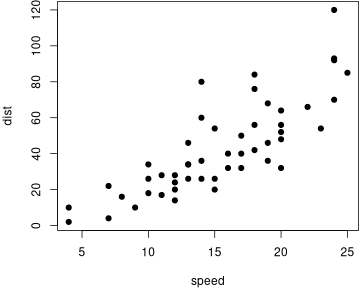
\includegraphics[width=\maxwidth]{/home/jek/test/cool-plot-1} \caption[A wonderful plot]{A wonderful plot.}\label{fig:cool-plot}
\end{figure}


\end{knitrout}

references:[]

bibliography::[]

appendix:[]

